\documentclass[12pt,letterpaper]{article}

\newenvironment{proof}{\noindent{\bf Proof:}}{\qed\bigskip}

\newtheorem{theorem}{Theorem}
\newtheorem{corollary}{Corollary}
\newtheorem{lemma}{Lemma} 
\newtheorem{claim}{Claim}
\newtheorem{fact}{Fact}
\newtheorem{definition}{Definition}
\newtheorem{assumption}{Assumption}
\newtheorem{observation}{Observation}
\newtheorem{example}{Example}
\newcommand{\qed}{\rule{7pt}{7pt}}

\newcommand{\assignment}[4]{
\thispagestyle{plain} 
\newpage
\setcounter{page}{1}
\noindent
\begin{center}
\framebox{ \vbox{ \hbox to 6.28in
{\bf CS412: ntroduction to Data Mining \hfill #1}
\vspace{4mm}
\hbox to 6.28in
{\hspace{2.5in}\large\mbox{Problem Set #2}}
\vspace{4mm}
\hbox to 6.28in
{{\it Handed Out: #3 \hfill Due: #4}}
}}
\end{center}
}

\newcommand{\solution}[4]{
\thispagestyle{plain} 
\newpage
\setcounter{page}{1}
\noindent
\begin{center}
\framebox{ \vbox{ \hbox to 6.28in
{\bf CS412:   Introduction to Data Mining \hfill #4}
\vspace{4mm}
\hbox to 6.28in
{\hspace{2.5in}\large\mbox{#3}}
\vspace{4mm}
\hbox to 6.28in
{#1 \hfill {\it #2}}
}}
\end{center}
\markright{#1}
}

\newenvironment{algorithm}
{\begin{center}
\begin{tabular}{|l|}
\hline
\begin{minipage}{1in}
\begin{tabbing}
\quad\=\qquad\=\qquad\=\qquad\=\qquad\=\qquad\=\qquad\=\kill}
{\end{tabbing}
\end{minipage} \\
\hline
\end{tabular}
\end{center}}

\def\Comment#1{\textsf{\textsl{$\langle\!\langle$#1\/$\rangle\!\rangle$}}}


%\documentclass{article}
\usepackage{amsmath}
\setlength{\parindent}{0pt}
\usepackage{graphicx}
%\usepackage{fullpage}
%\usepackage{setspace} 
\usepackage{float}
%\usepackage{listings} 
%\usepackage{bbm}
\usepackage{bigstrut}
%\usepackage{caption}
%\usepackage{subcaption}
%\usepackage{algpseudocode}
%\usepackage{algorithm}

\usepackage{listings}
\usepackage{color}
\usepackage[utf8]{inputenc}

\definecolor{dkgreen}{rgb}{0,0.6,0}
\definecolor{gray}{rgb}{0.5,0.5,0.5}
\definecolor{mauve}{rgb}{0.58,0,0.82}

\lstset{frame=tb,
  language=matlab,
  aboveskip=3mm,
  belowskip=3mm,
  showstringspaces=false,
  columns=flexible,
  basicstyle={\small\ttfamily},
  numbers=none,
  numberstyle=\tiny\color{gray},
  keywordstyle=\color{blue},
  commentstyle=\color{dkgreen},
  stringstyle=\color{mauve},
  breaklines=true,
  breakatwhitespace=true,
  tabsize=3
}


\oddsidemargin 0in
\evensidemargin 0in
\textwidth 6.5in
\topmargin -0.5in
\textheight 9.0in
\usepackage{multirow}
\usepackage{hyperref}

\hypersetup{colorlinks=true}
\usepackage{color}

%\newcommand{\ans}[1]{{[{\sc Answer:} {\sf #1}]}}
\newcommand{\ans}[1]{}


\begin{document}


\solution{Li Miao}{\today}{Assignment 2}{Fall 2015}
% Fill in the above, for example, as follows:
% \solution{Joe Smith}{\today}{1}{Fall 2012}


\section*{Question 1 (16 points)}
Assume that a base cuboid of 6 dimensions contains only 3 base cells:
\begin{center}
$(a_1, a_2, a_3, a_4,a_5,a_6)$, $(b_1, b_2, a_3, a_4,a_5,a_6)$, and $(c_1, c_2, a_3, a_4,a_5,a_6)$
\end{center}
where $a_i \neq b_i$, $b_i \neq c_i$, and $a_i \neq c_i$,  $\forall i = 1,2$. There is no dimension with concept hierarchy. The measure of the cube is {\it count}. The {\it count} of each base cell is $1$.\\

{\bf Requirements}
\begin{itemize}\vspace{-2mm}\setlength\itemsep{0mm}
\item Include final results and explain how you calculate the cells in the Answer Document. Keep it brief and clear.
\end{itemize}
\begin{itemize}
\item[a.]  $2^6 = 64$. 
\item[b.] $2^4 * (3*2^2 -2) -3 = 157$. For last four dimensions, we have only two choice (include $*$). Then for first two dimensions, we need to discuss 3 conditions. $a_1,*,a_2,*$,$b_1,*,b_2,*$,$c_1,*,c_2,*$. And we need to delete the 2 overlap of $*$. Finally, we need to delete the 3 base cells. 
\item[c.]  $2^4 = 16$. Only when first two dimensions are both stars. 
\item[d.]  4. First two dimensions are stars, left 4 dimensions are not stars.
\end{itemize}

\section*{Question 2 (24 points)}
We give you an artificially generated dataset \texttt{Data-Q2.txt} in the dataset file. It contains 100 business records. Each row is a business record, and the data fields in each row are separated by tabs. Each record contains the fields \texttt{Business\_ID}, \texttt{City}, \texttt{State}, \texttt{Category}, \texttt{Price}, \texttt{Quarter}, \texttt{Year}. The four quarters in a year are denoted $Q1$, $Q2$, $Q3$ and $Q4$. We now want to construct a cube over the 4 dimensions \texttt{Location}, \texttt{Category}, \texttt{Price}, and \texttt{Time}, with {\it count} as the measure. The \texttt{Location} dimension has a \texttt{City-State} concept hierarchy and, similarly, the \texttt{Time} dimension has a \texttt{Quarter-Year} hierarchy.\\
\begin{itemize}
\item[a.] (4', L1) T = $(2+1)*(1+1)*(1+1)*(2+1) = 36$
\item[b.] (4', L2) 56.
\item[c.] (4', L2) 34.
\item[d.] (4', L2) 33.
\item[e.] (4', L2) 10.
\item[f.] (4', L2) 4.
\end{itemize}

\section*{Question 3 (15 points)}
\begin{figure}[t]
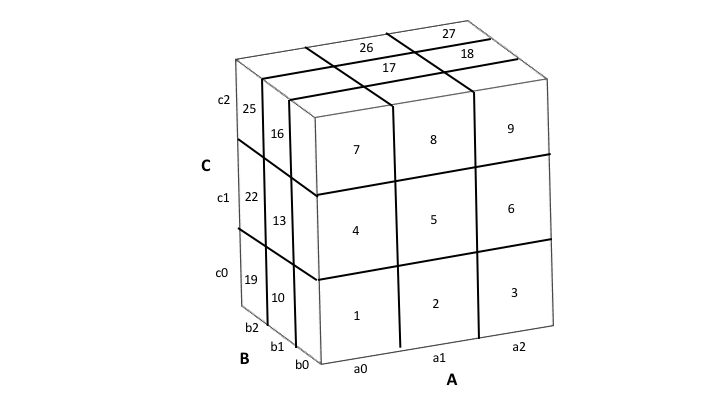
\includegraphics[width=0.8\textwidth]{Figures/fig-chunk.png}
\centering
\caption{A 3-D array with dimensions $A$, $B$ and $C$. This array is divided into 27 smaller chunks.}
\label{fig:chunk}
\end{figure}
We have a data array with 3 dimensions $A$, $B$ and $C$. The 3-D array is divided into small chunks. Each dimension is divided into 3 equally sized partitions. See Figure~\ref{fig:chunk}. For example, dimension $A$ is divided into $a_0$, $a_1$, and $a_2$, and dimension $B$ is divided into $b_0$, $b_1$, and $b_2$. There are totally 27 chunks and each chunk is denoted by $a_ib_jc_k$. The sizes of the dimensions $A$, $B$, and $C$ are 900, 300, and 600. Since we divide each dimension into 3 parts with equal size, the sizes of the chunks on dimensions $A$, $B$, and $C$ are 300, 100, and 200 respectively. Now we want to use \textbf{Multiway Array Aggregation Computation} to materialize the 2-D cuboids $AB$, $AC$ and $BC$.\\


\begin{itemize}
\item[a.] (7', L2) 
For 2-D planes, we need to keep 1 BC, 3 AB and 9 AC chunks in memory per period.

So the size is $BC+3AB+9AC = 100*200 + 3*300*100 + 9 * 300*200 = 650000$. 
\item [b.] (8', L3) 
Yes. There exist other orders to scan the chunks so that the memory cost is less than that in sub-question (a).
We hope to keep as few AC as possible because the size of AC chunk is larger than others, AB and BC. So we hope to scan AC only 1 time per run time. And we can scan the whole BC plane because the size of its chunk is the smallest in three 2-D planes. 

Therefore, we can do this following order:
1-10-19

4-13-22

7-16-25

2-11-28

5-14-23

8-17-26

3-12-21

6-15-24

9-18-27

Then we need to keep 1 AC, 3 AB, 9 BC chunks in memory per period.
The size is $300*200+3*300*100+9*200*100=330000$. 



\end{itemize}

\section*{Question 4 (15 points)}
We have a 3-D data array with 3 dimensions $A, B, C$. The data contained in the array is as follows:\\
\begin{align*}
(a_0,b_0,c_0): 1 & ~ &  (a_0,b_0,c_1): 1 & ~ &  (a_0,b_0,c_2): 1  \\
(a_0,b_1,c_0): 1 & ~ &  (a_0,b_1,c_1): 1  & ~ &  (a_0,b_1,c_2): 1\\
(a_0,b_2,c_0): 1 & ~ &  (a_0,b_2,c_1): 1 & ~ &  (a_0,b_2,c_2): 1 \\
(a_0,b_3,c_0): 1 & ~ &  (a_0,b_3,c_1): 1 & ~ &  (a_0,b_3,c_2): 1
\end{align*}
You will use the \textbf{Bottom-Up Computation (BUC)} algorithm to materialize the cube. Please answer the following questions.\\
\begin{itemize}

\item[a.] 
\begin{figure}[H]
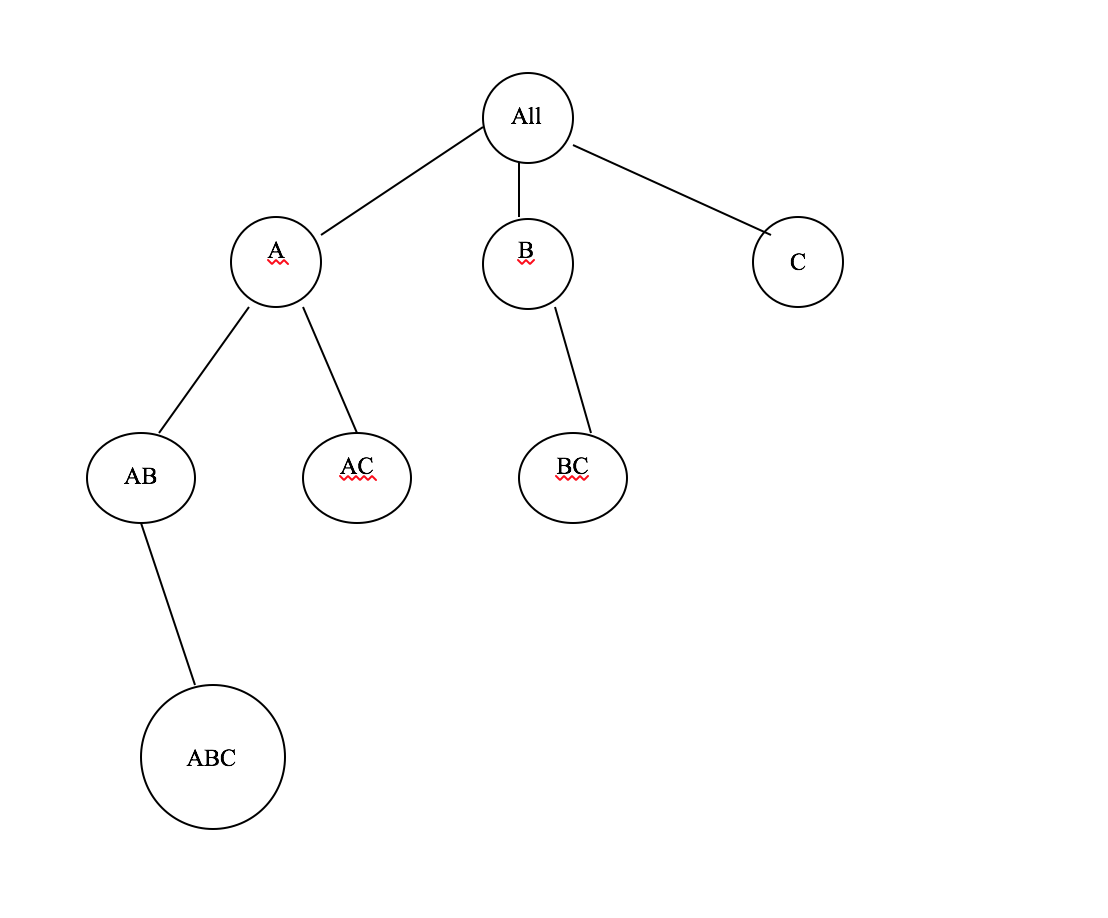
\includegraphics[width=0.8\textwidth]{Figures/treetrace.png}
\centering
\caption{trace tree of expansion with the exploration order $A\rightarrow B \rightarrow C$}
\label{fig:tree}
\end{figure}

\item[b.] (5', L3) 16 cells will be considered. 

All($*,*,*$):12 - expansion

\underline{\hspace{ 1in}}

A($a_0$,$*$,$*$):12 - expansion

\underline{\hspace{ 1in}}

AB($a_0,b_0,*$):3\\
AB($a_0,b_1,*$):3\\
AB($a_0,b_2,*$):3\\
AB($a_0,b_3,*$):3

\underline{\hspace{ 1in}}

AC($a_0,*,c_0$):4\\
AC($a_0,*,c_1$):4\\
AC($a_0,*,c_2$):4

\underline{\hspace{ 1in}}

B($*,b_0,*$):3\\
B($*,b_1,*$):3\\
B($*,b_2,*$):3\\
B($*,b_3,*$):3

\underline{\hspace{ 1in}}

C($*,*,c_0$):4\\
C($*,*,c_1$):4\\
C($*,*,c_2$):4\\

\item[c.] (5', L3) If we set $min\_support = 4$ with the exploration order $B \rightarrow A \rightarrow C$, 12 cells would be considered.\\
All($*,*,*$):12 - expansion

\underline{\hspace{ 1in}}

B($*,b_0,*$):3\\
B($*,b_1,*$):3\\
B($*,b_2,*$):3\\
B($*,b_3,*$):3

\underline{\hspace{ 1in}}

A($a_0$,$*$,$*$):12 - expansion

\underline{\hspace{ 1in}}

AC($a_0,*,c_0$):4\\
AC($a_0,*,c_1$):4\\
AC($a_0,*,c_2$):4

\underline{\hspace{ 1in}}

C($*,*,c_0$):4\\
C($*,*,c_1$):4\\
C($*,*,c_2$):4\\

\end{itemize}


\section*{Question 5 (10 points)}
\begin{itemize}
\item[a.] \textbf{F.}  Static Status: operational update of data does not occur in the data warehouse environment.
\item[b.] \textbf{F.}  Cell $B$ is a child of cell $A$.
\item[c.] \textbf{F.}  In OLAP operations, we can see more general data information by rolling up.
\item[d.] \textbf{T.}  The Bottom-Up Computation (BUC) algorithm can be used to compute either the full cube or a partial cube. If {min\_sup} = 1, then the full Cube. If partition does not satisfy {min\_sup}, it decedents can be pruned.
\item[e.] \textbf{F.} The Multiway Array Aggregation Computation is most effective when the product of the cardinalities of dimensions is low.
\end{itemize}

\newpage


\section*{Mini Machine Problem (20 points)}
CubesViewer is a visual, web-based tool application for exploring and analyzing OLAP databases served by the Cubes OLAP Framework\footnote{https://github.com/jjmontesl/cubesviewer}. The CubesViewer Explorer demo can be found at \url{http://crow.cs.illinois.edu:8080/cubesviewer/}. You can login with user {\tt cs412}, password {\tt cs412f2015}\\
  
\begin{enumerate}
\item[a.](5', L2) 
Mountain Bike has the highest revenue. Termic Jacket has the least revenue. \\
Steps: Drill down:Country:Region $\rightarrow$ 
Drill down:Sale Date/Monthly:Year $\rightarrow$ 
Drilldown:Product:Category $\rightarrow$ 
Slice:Country:Region = Europe $\rightarrow$ 
Slice:Sale Date/Monthly:Year = 2012 $\rightarrow$
 Slice:Product:Category = Sports $\rightarrow$ 
 Drilldown:Product:Product $\rightarrow$ 
 Dice:Sale Date/Monthly:Year = 2012,1;2012,2;2012,3
\begin{figure}[H]
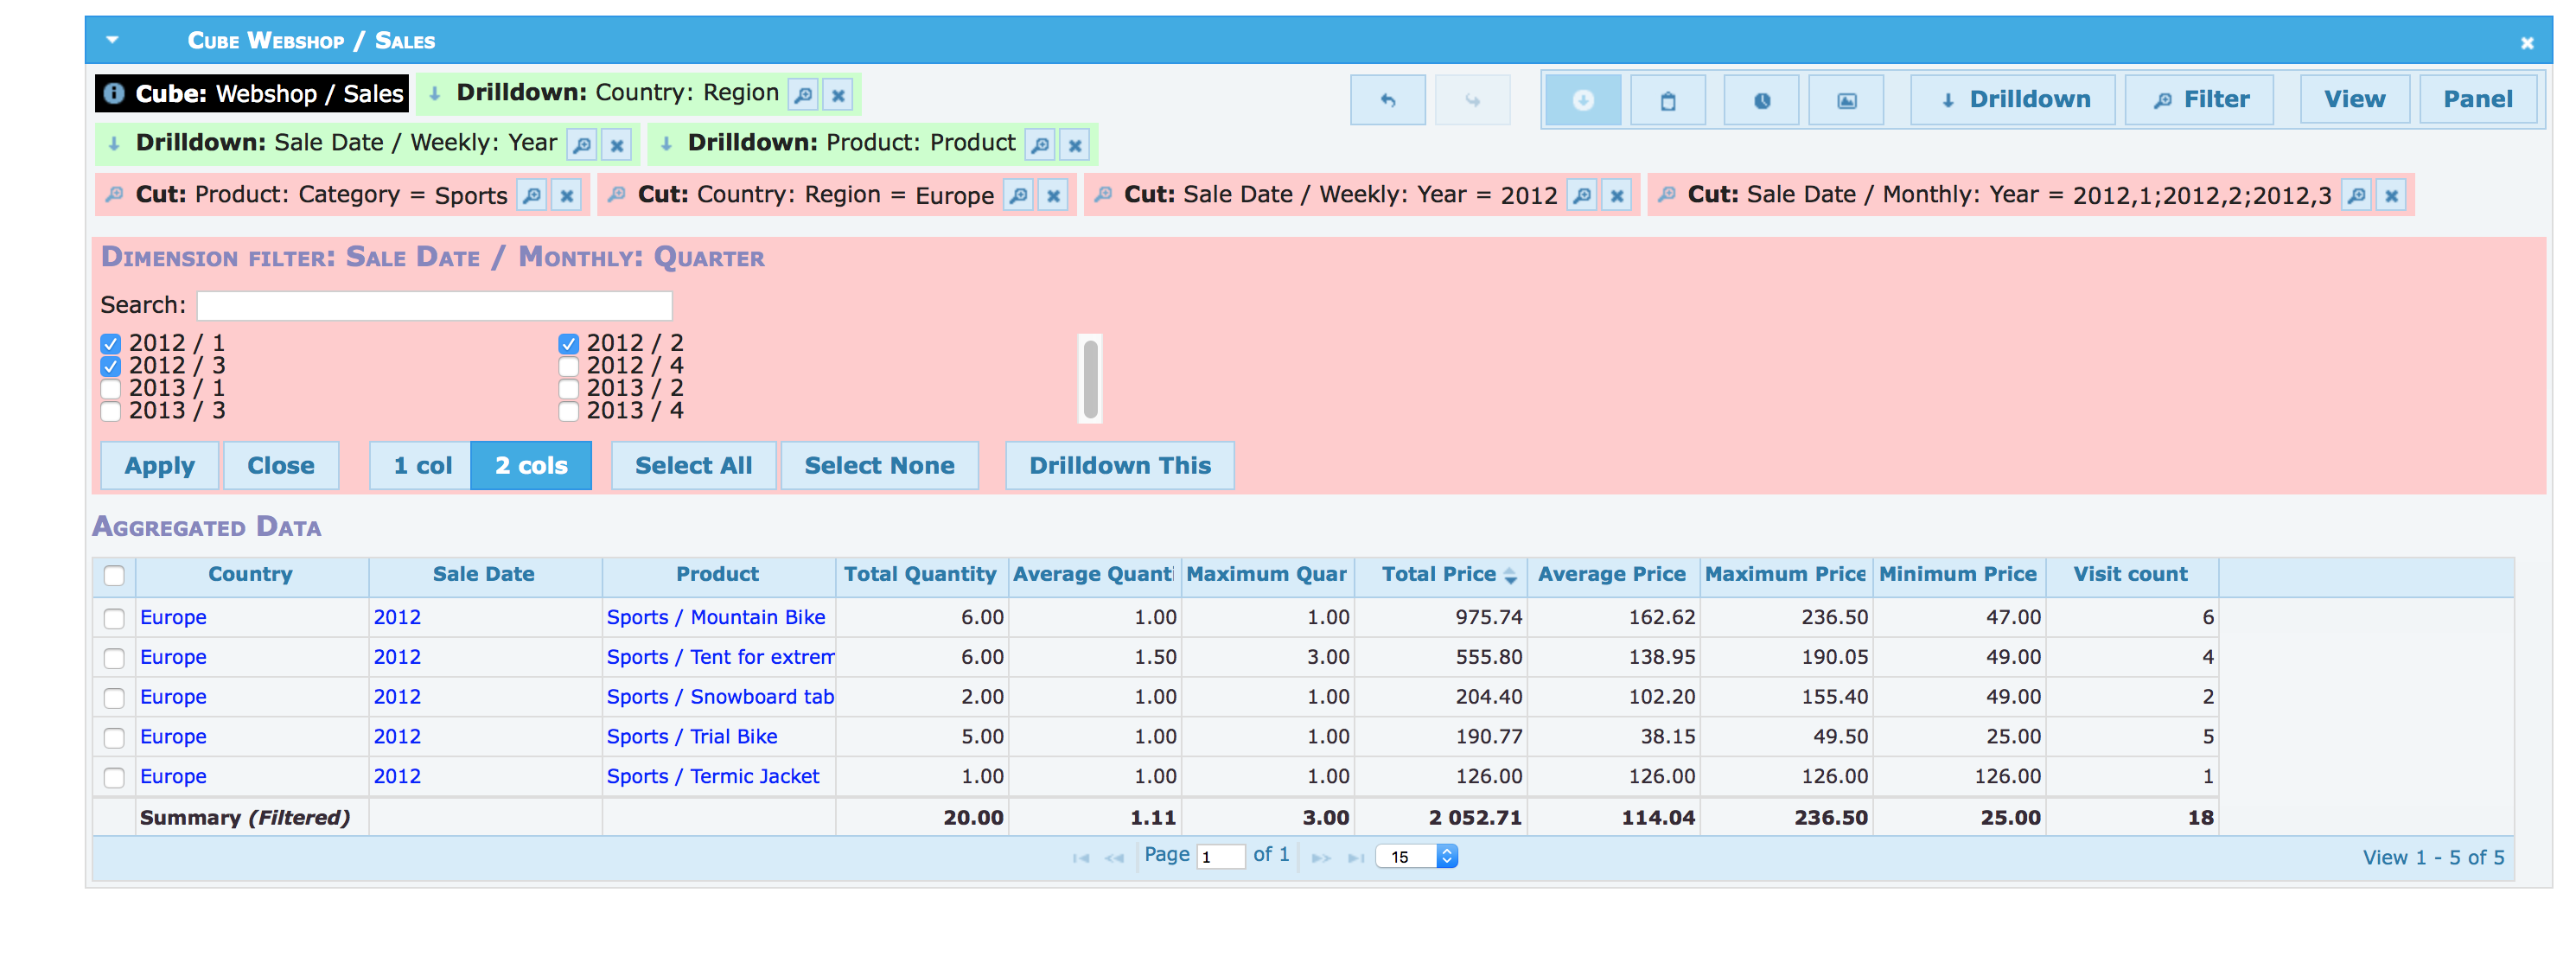
\includegraphics[width=0.8\textwidth]{Figures/5a.png}
\centering
%\caption{trace tree of expansion with the exploration order $A\rightarrow B \rightarrow C$}
%\label{fig:tree}
\end{figure}

\begin{figure}[H]
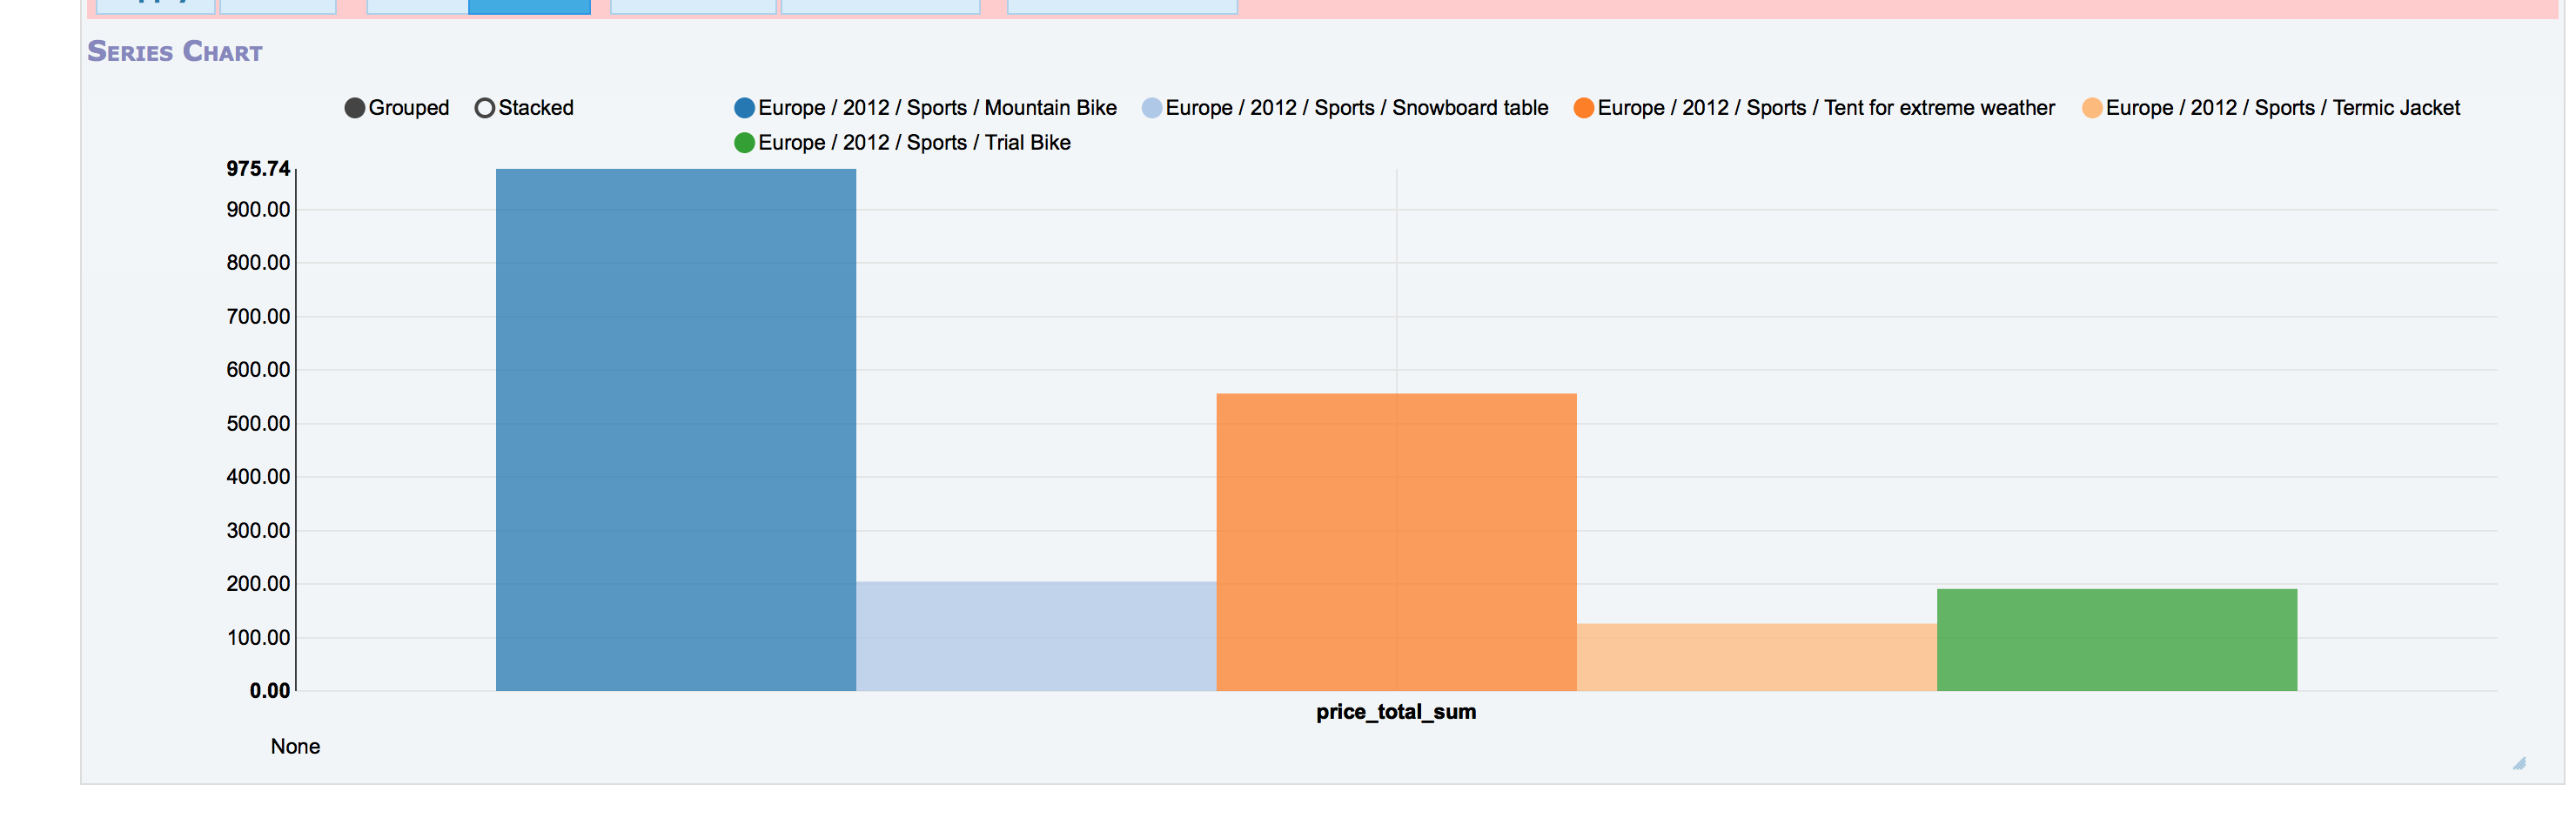
\includegraphics[width=0.8\textwidth]{Figures/5a2.png}
\centering
%\caption{trace tree of expansion with the exploration order $A\rightarrow B \rightarrow C$}
%\label{fig:tree}
\end{figure}

\item[b.](4', L2)
Use web search in chrome is the popular way in North America.\\
Steps: Drilldown: Country;Region $\rightarrow$ 
Drilldown: source$\rightarrow$ 
Drilldown:Browser $\rightarrow$
 Slice: Country:Region={North\_America}\\
\begin{figure}[H]
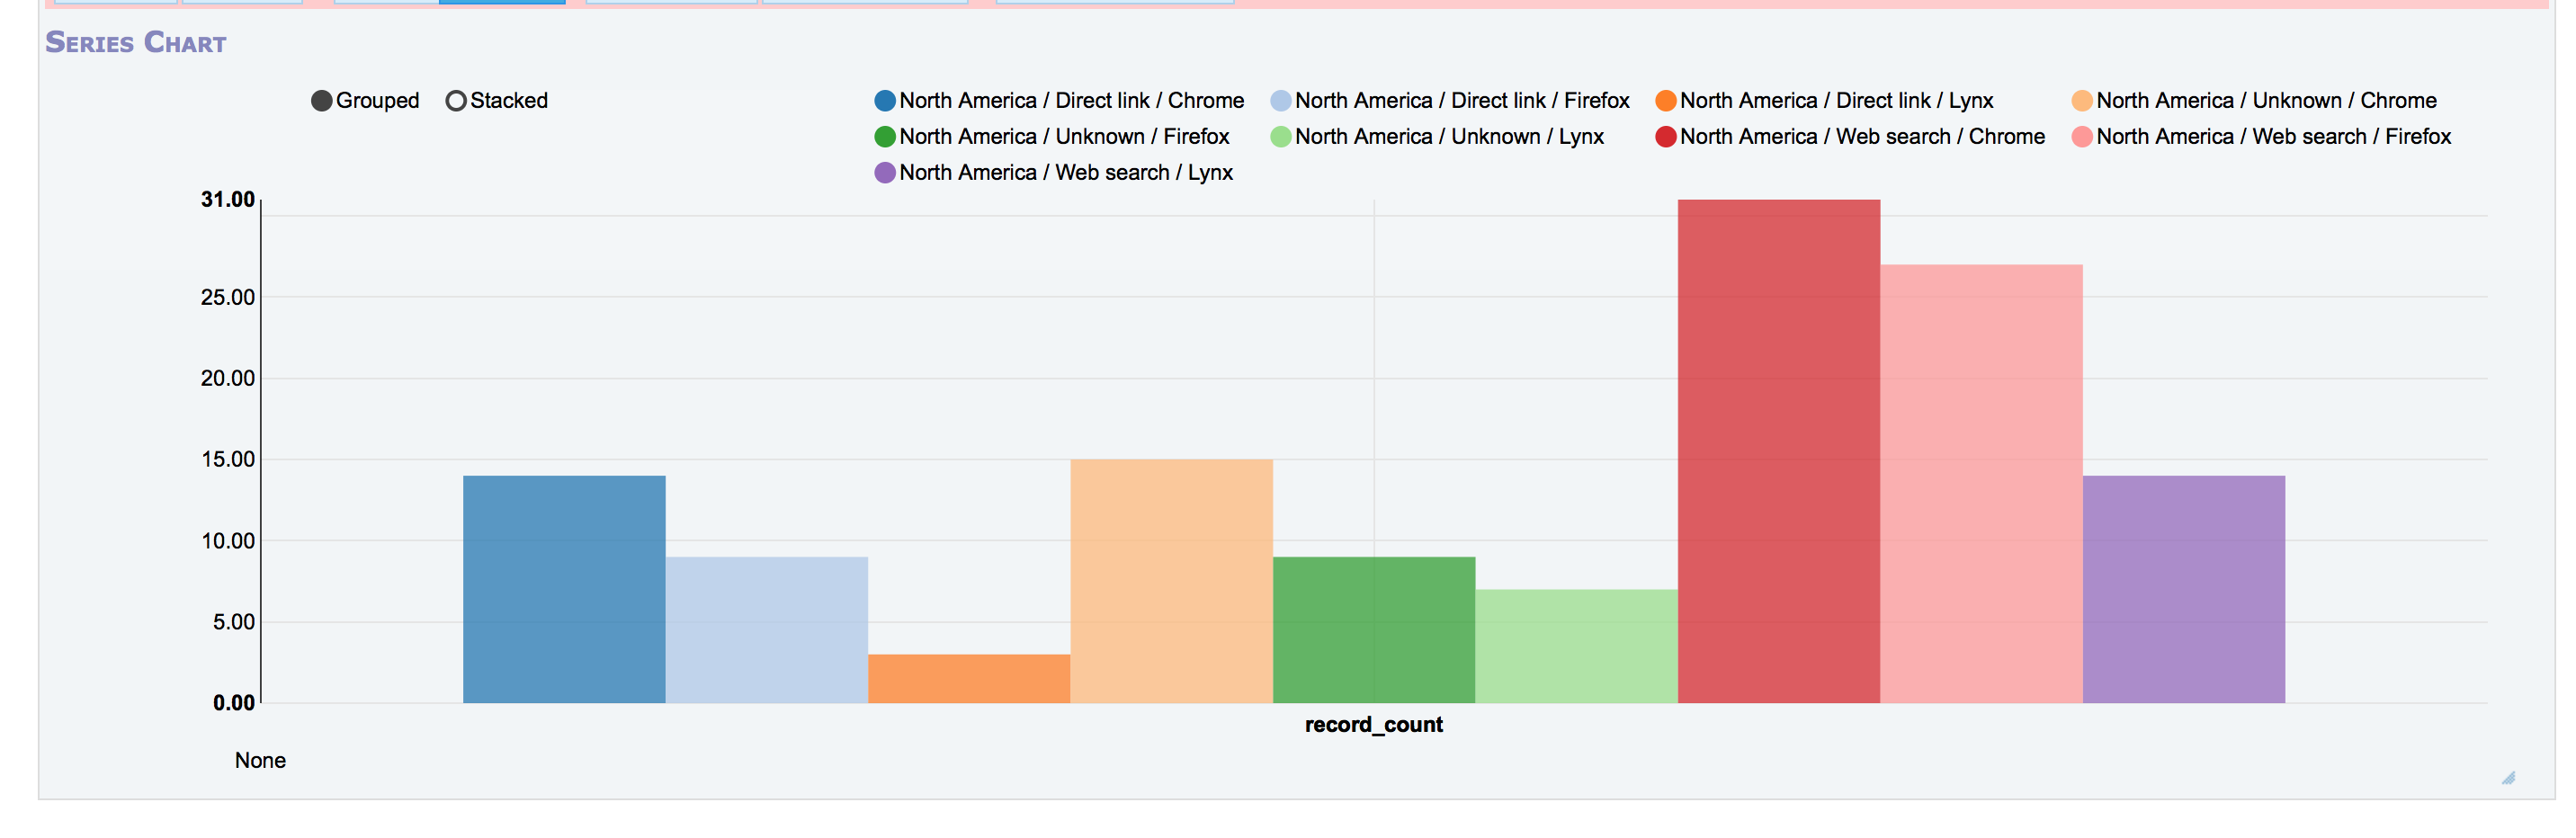
\includegraphics[width=0.8\textwidth]{Figures/5b.png}
\centering
%\caption{trace tree of expansion with the exploration order $A\rightarrow B \rightarrow C$}
%\label{fig:tree}
\end{figure}

\item[c.](3', L2) 
\begin{figure}[H]
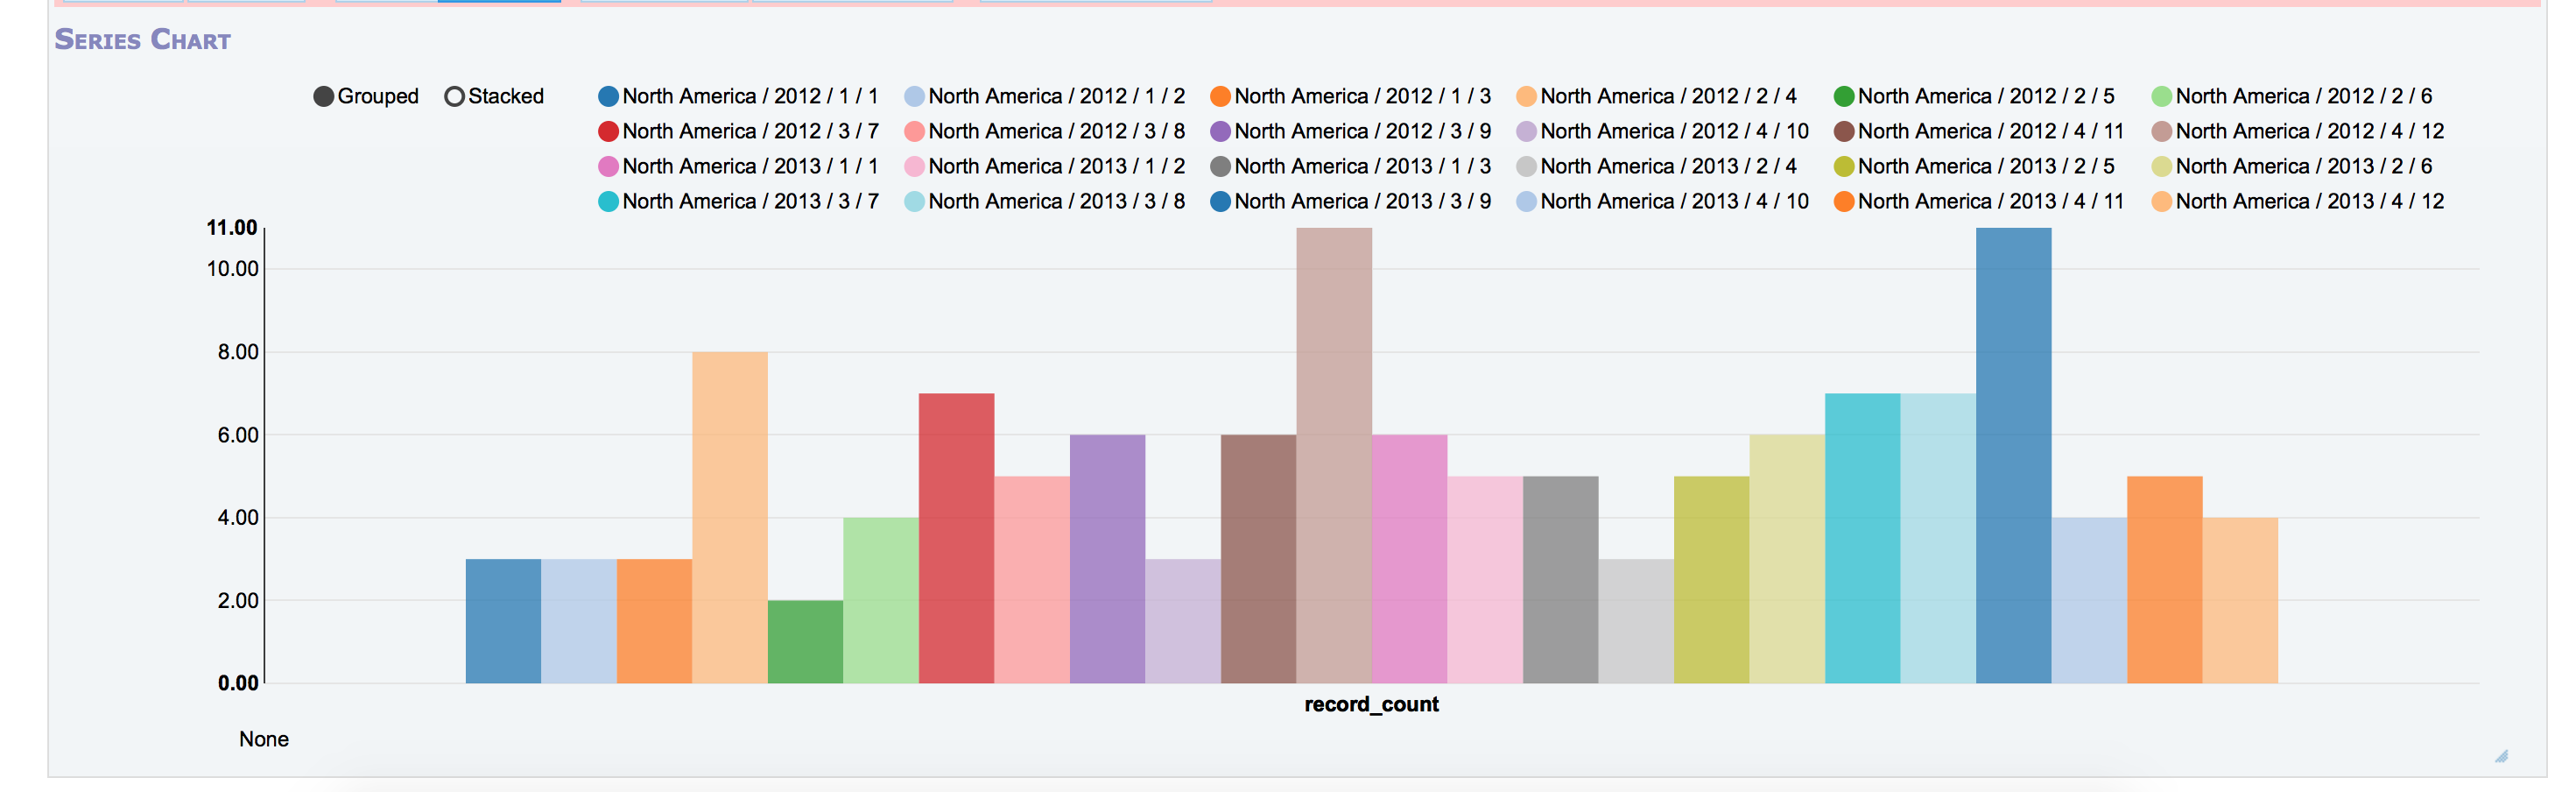
\includegraphics[width=0.8\textwidth]{Figures/5c1.png}
\centering
%\caption{trace tree of expansion with the exploration order $A\rightarrow B \rightarrow C$}
%\label{fig:tree}
\end{figure}

\item[d.](8', L3)
\begin{itemize}
\item Webshop/Sales
Steps: Drilldown:Country:Region$\rightarrow$
Drilldown:Sale Date/Monthly:Year
$\rightarrow$Drilldown:Product:Product 
$\rightarrow$Slice:Country:Region={North\_America} 
$\rightarrow$ Slice: Year = 2013

\begin{figure}[H]
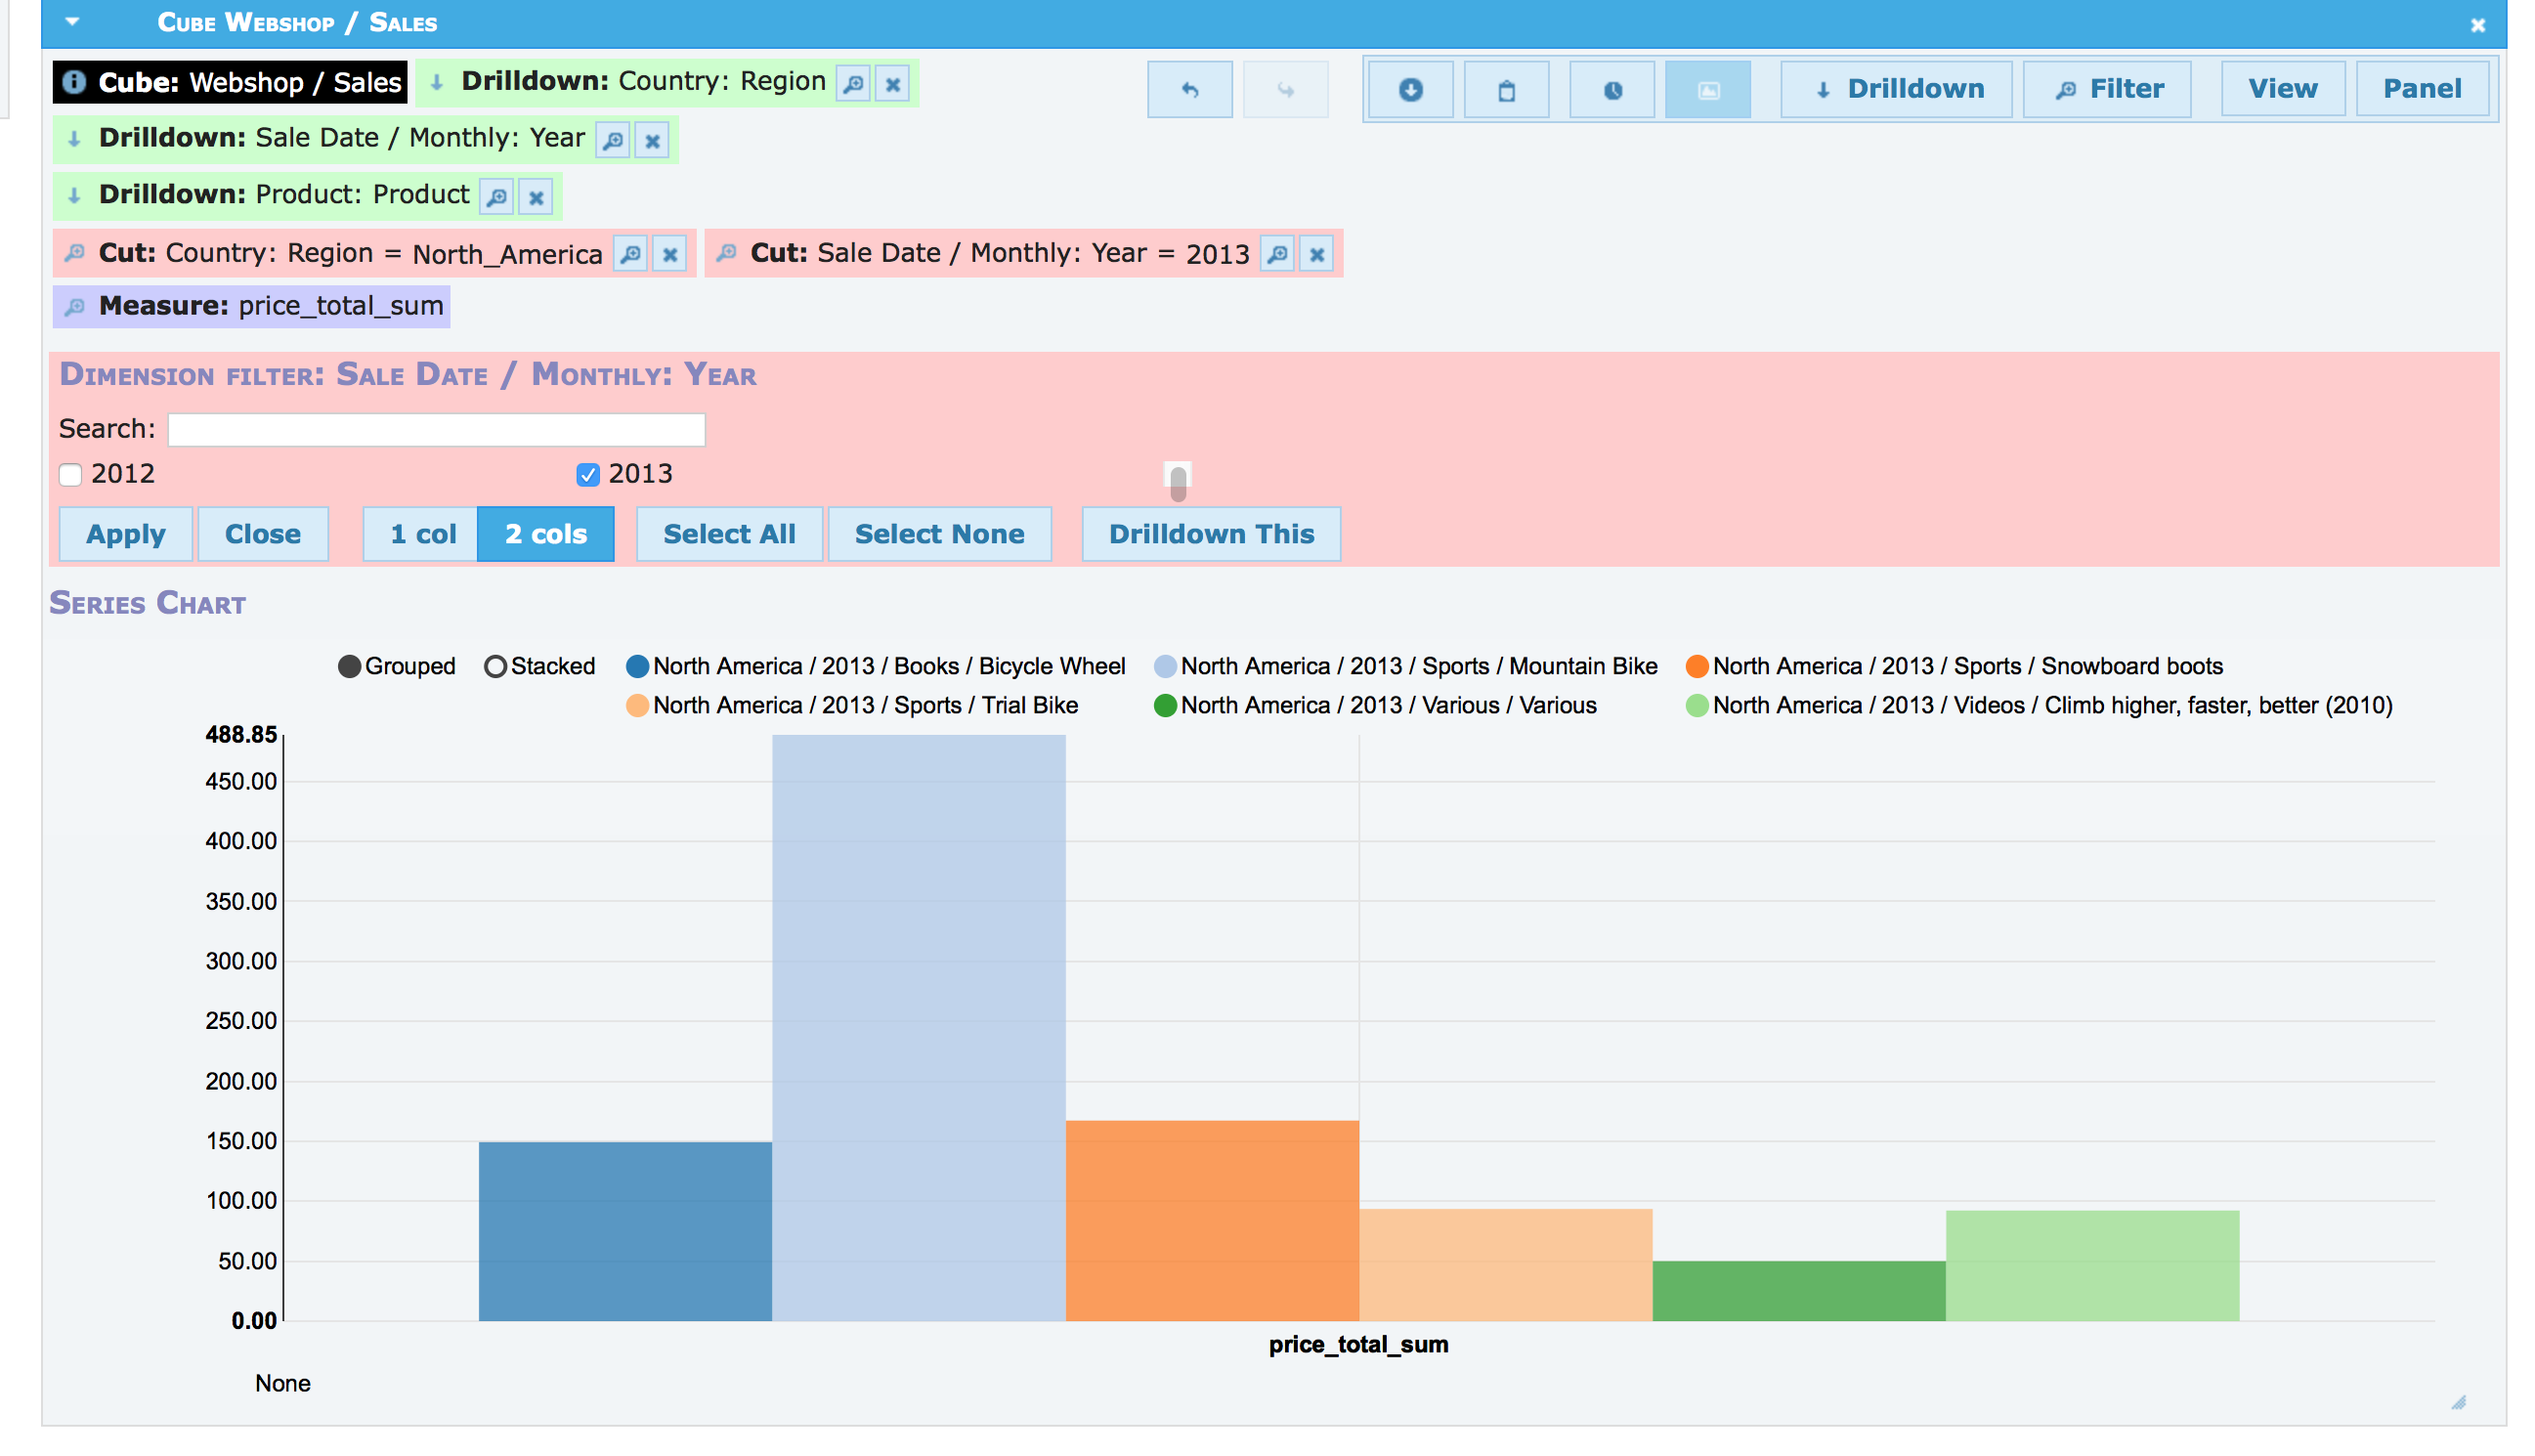
\includegraphics[width=0.8\textwidth]{Figures/d1.png}
\centering
%\caption{trace tree of expansion with the exploration order $A\rightarrow B \rightarrow C$}
%\label{fig:tree}
\end{figure}

Therefore, in North America 2013, the Mountain Bike in sports has the highest avenue. So we should restock more Mountain Bike.


\item Website/Visits
Steps: DrilldownCountry:Country$\rightarrow$
Drilldown:Source$\rightarrow$
Drilldown:Browser$\rightarrow$
Slice: Country:Region = {North\_America,United\_States\_of\_America}


\begin{figure}[H]
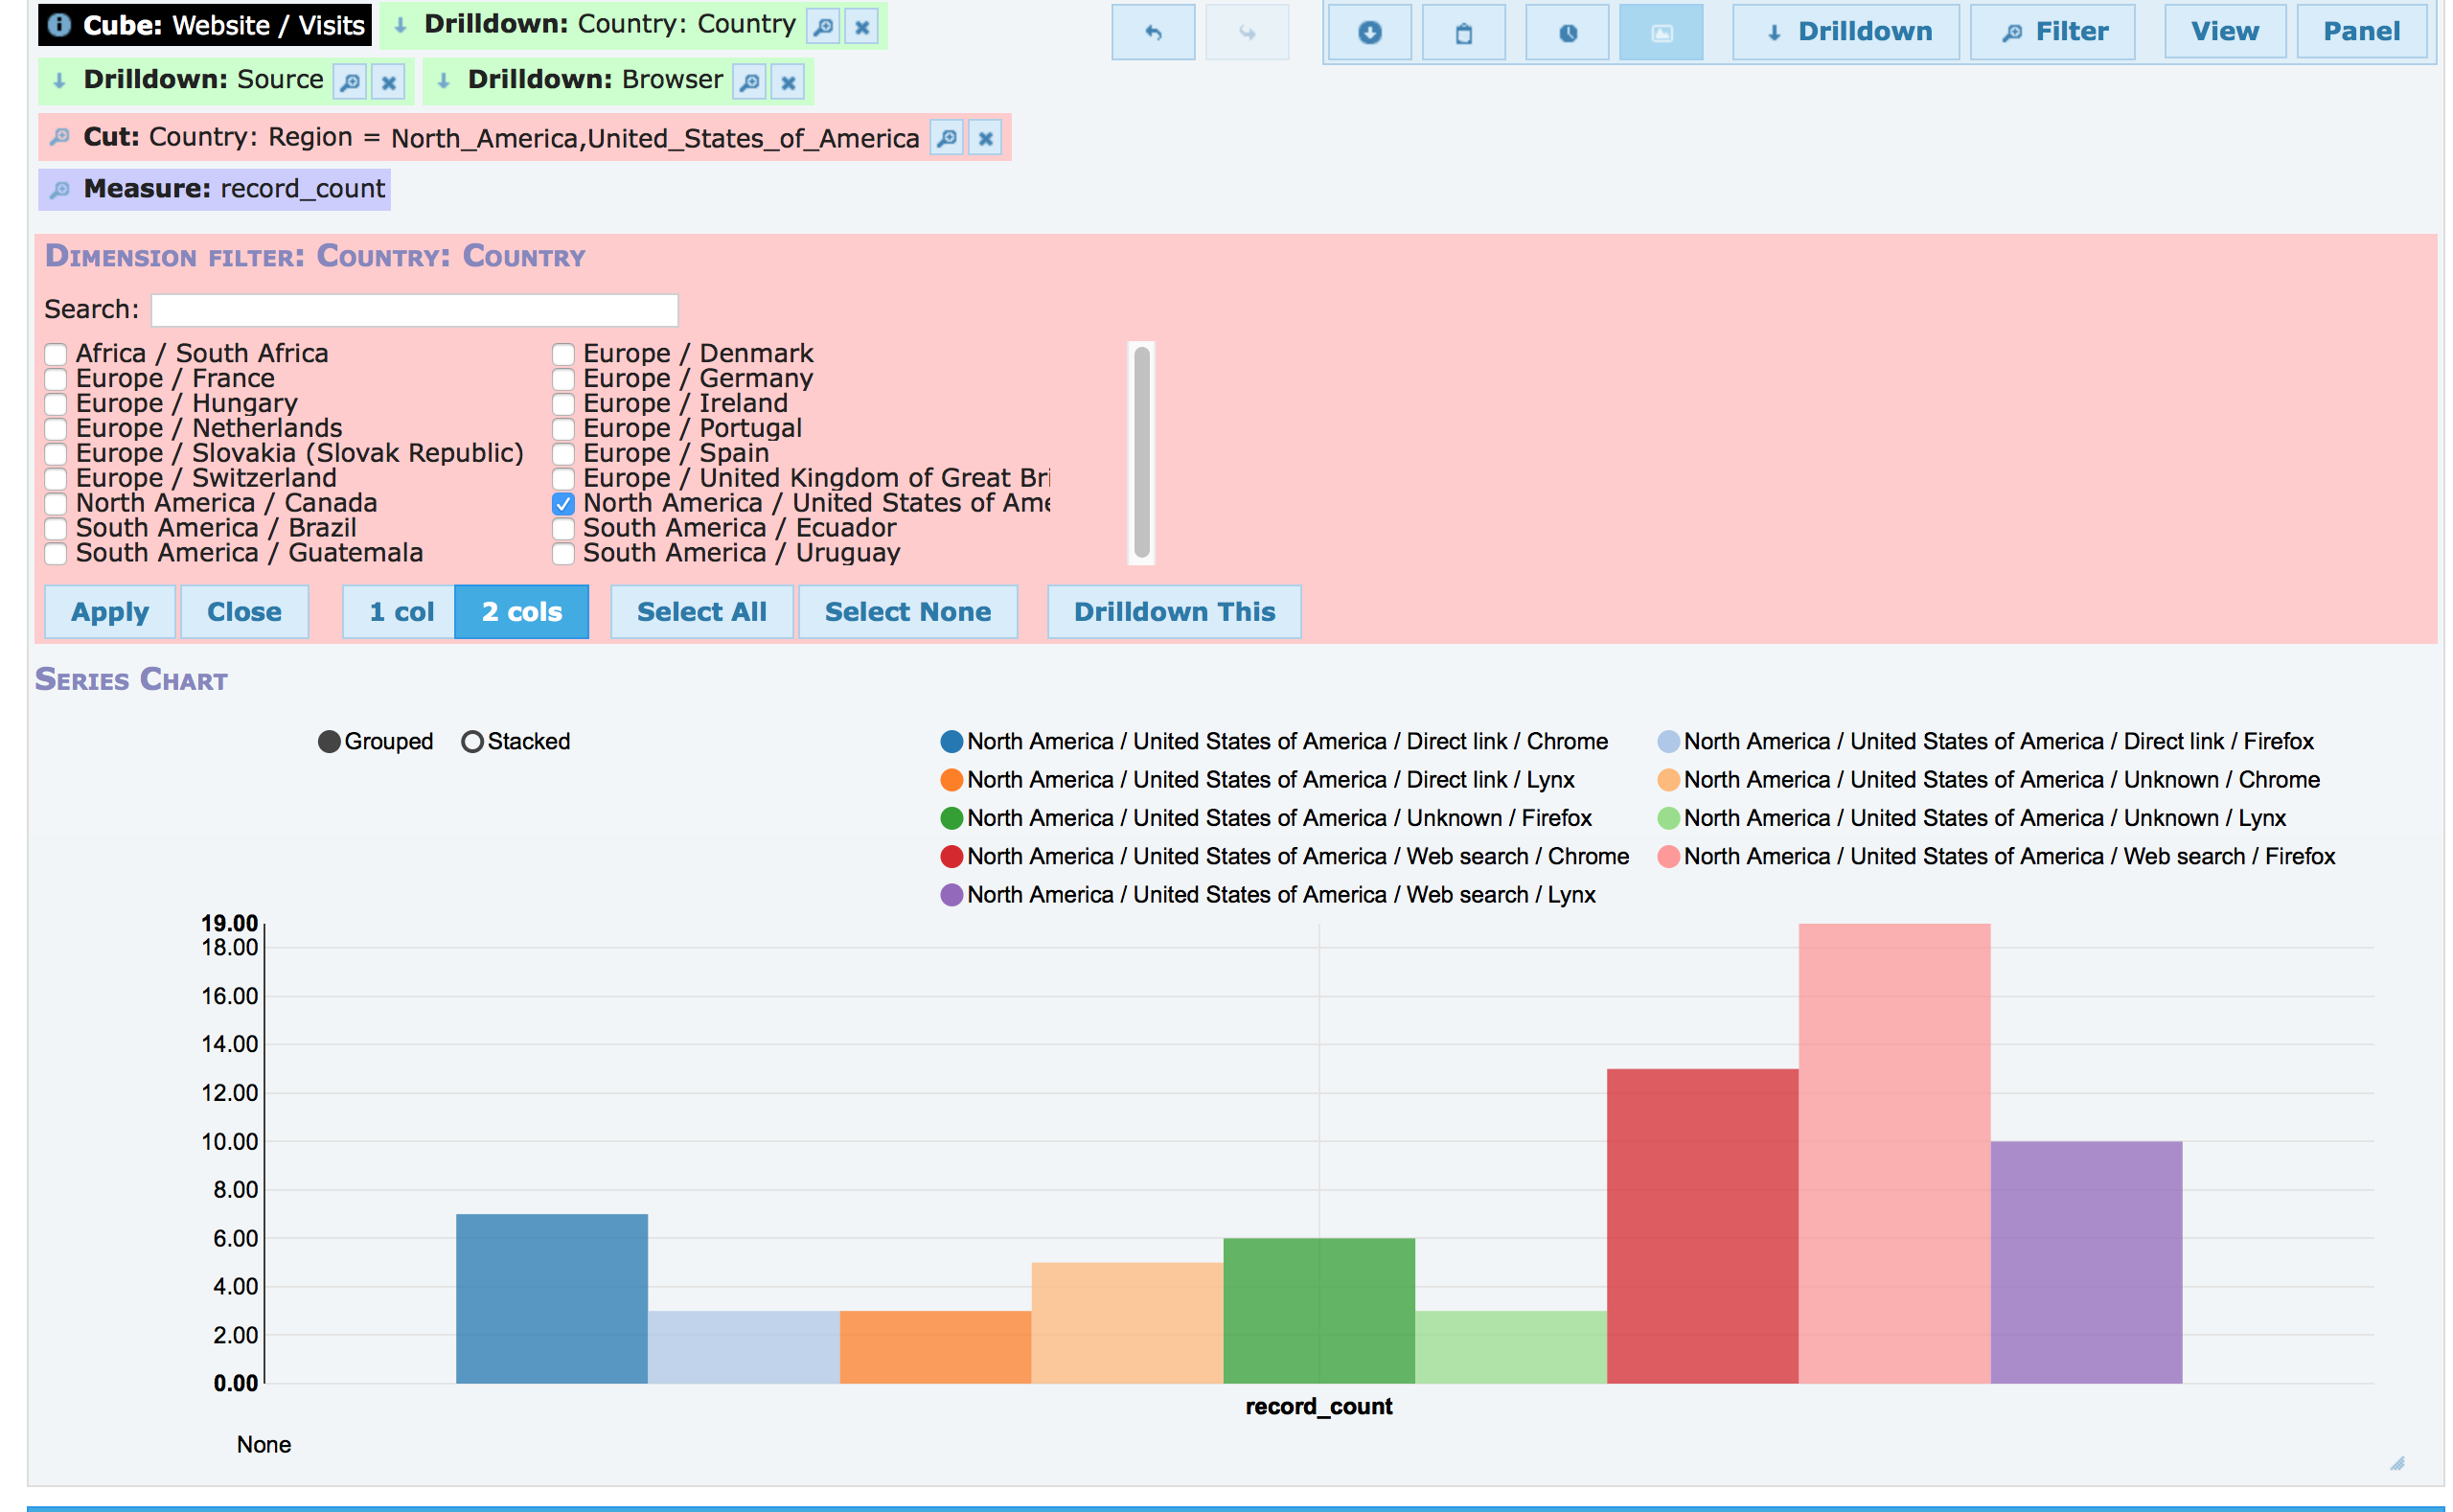
\includegraphics[width=0.8\textwidth]{Figures/d2.png}
\centering
%\caption{trace tree of expansion with the exploration order $A\rightarrow B \rightarrow C$}
%\label{fig:tree}
\end{figure}

Therefore, In United States of America, the most popular way for customers to visit online store is by web search on Firefox. So we should invest more ads on Firefox to attract more customers. 

\end{itemize}

\end{enumerate}


\end{document}